\documentclass[10pt]{article}
\usepackage{../local}


\newcommand{\classcode}{Physics 110A}
\newcommand{\classname}{Electromagnetism and Optics}
\renewcommand{\maketitle}{%
\hrule height4pt
\large{Eric Du \hfill \classcode}
\newline
\large{HW 02} \large{\hfill \classname \hfill} \large{\today}
\hrule height4pt \vskip .7em
\normalsize
}
\linespread{1.1}
\begin{document}
    \maketitle
    
    \section*{Collaborators}

    I worked with \textbf{Andrew Binder, Christine Zhang, Teja Nivarthi} on this assignment. 

    \section*{Problem 1}

    The electric field of a solid sphere with radius $R$ and uniform charge density $\rho$ is given by 
    \begin{equation}
        \mathbf E = \begin{cases}
        \dfrac{\rho \mathbf r}{3\epsilon_0} & (r < R)\\\\
        \dfrac{kQ}{r^2} \mathbf{\hat r} & (r > R)
    \end{cases}
    \end{equation}
    where $Q$ is the total charge of the sphere. The magnetic field of an infinitely long thick table with radius $a$ is given by 
    \[ \mathbf B = \begin{cases}
        \dfrac{\mu_0 Js}{2} \hat \phi & (s < a)\\\\
        \dfrac{\mu_0I}{2\pi s} \hat \phi & (s > a)
    \end{cases}\]
    where the net current $I$ flows in the $+z$-direction. Note that the $\mathbf E$-field and $\mathbf B$-field are expressed in spherical and cylindrical coordinates respectively. 
    \begin{enumerate}[label=(\alph*), start]
        \item Calculate the divergence and curl of $\mathbf E$ with spherical coordinates

        \begin{solution}
            Firstly, there's no $\theta$ or $\phi$ dependence, so we only care about the $r$ part of the divergence, so for $r < R$,
            \[ \div \mathbf E = \frac{1}{r^2}\pdv{r}\left(r^2 \frac{\rho}{3\epsilon_0}\right) = \frac{1}{r^2} \frac{\rho}{3\epsilon_0} \cdot 2r = \frac{2\rho}{3\epsilon_0r}\]
            Then for $r > R$: 
            \[ \div \mathbf E = \frac{1}{r^2} \pdv{r} \left( r^2 \frac{kQ}{r^2}\right) =  \frac{1}{r^2} \pdv{r}\left( kQ\right) = 0\]
            Therefore, we can write:
            \[ \div \mathbf E = \begin{cases}
                \dfrac{2\rho}{3\epsilon_0 r} & (r < R)\\
                0 & (r > R)
            \end{cases}\]
            The electric field has no $\theta$ or $\phi$ component anywhere, so therefore $\curl \mathbf E = 0$ for both regimes $r < R$ and $r > R$. 
        \end{solution}
        \item Calculate the divergence and curl of $\mathbf B$ in cylindrical coordinates.
        
        \begin{solution}
            Just like the previous part, we know that since $\mathbf B$ only has a $\phi$ component for $s < a$: 
            \[ \div \mathbf B = \frac{1}{s} \pdv{B_{\phi}}{\phi} = \frac 1s \pdv{\phi}\left( \frac{\mu_0 Js}{2}\hat \phi \right) = 0\] 
            We also have for $s > a$: 
            \[ \div \mathbf B = 0\]
            For the curl, we know that the curl takes on the general form: 
            \[ \curl \mathbf v = \left( \frac 1s \pdv{v_z}{\phi} - \pdv{v_\phi}{z}\right) \hat s + \left( \pdv{v_s}{z} - \pdv{v_z}{s}\right) \hat \phi + \frac 1s\left[\pdv{s}(s v_\phi) - \pdv{v_s}{\phi}\right]\hat z\]
            $\mathbf B$ has no $\theta$ or $\phi$ component, so only the $\hat z$ component survives. For $s < a$: 
            \[ \curl \mathbf B = \frac 1s \left[ \pdv{s}\left( \frac{s \mu_0 J s}{2}\right) \right] \hat z = \frac 1s \left[ \frac{\mu_0 J}{2} \cdot 2s\right] \hat z = \mu_0 J \hat z\]
            and likewise for $s > a$: 
            \[ \curl \mathbf B = \frac 1s\left[ \pdv{s}\left( s \cdot \frac{\mu_0 I}{2\pi s}\right) \right] \hat z = \frac 1s \left[\pdv{s}(\mu_0 I)\right]\hat z = 0\] 
            And so therefore:
            \[ \curl \mathbf B = \begin{cases}
                \mu_0 J \hat z & (s < a)\\
                0 & (s > a)
            \end{cases}\]
        \end{solution}
    \end{enumerate}

    Independent of the previous part, consider a vector field $\mathbf V = s(2 + \cos^2 \phi) \hat s + s \sin \phi \cos \phi \mathbf{ \hat \phi} + 3z \hat z$.

    \begin{enumerate}[label= (\alph*), resume]
        \item Calculate the divergence and curl of the vector $\mathbf V$. 

        \begin{solution}
            Here we use the full form of the divergence. We then get: 
            \begin{align*}
                \div \mathbf V &= \frac 1s \pdv{s} (s \cdot 2\cos^2 \phi) + \frac 1s \pdv{\phi}(s \sin \phi \cos \phi) + \pdv{z} (3z)\\
                &= 2\cos^2 \phi + (\cos^2 \phi - \sin^2 \phi) + 3 \\
                &= 2\cos^2 \phi + \cos(2\phi) + 7
            \end{align*}
            Similarly with the curl: 
            \begin{multline*}
                \curl \mathbf V = \left( \frac1s \pdv{\phi}(3z) - \pdv{z} (s \sin \phi \cos \phi)\right)  \hat s + \left(\pdv{z} \left( s \cdot 2\cos^2 \phi\right) - \pdv{s}(3z)\right) \hat \phi \\ + \frac 1s \left( \pdv{s}(s^2 \sin \phi \cos \phi) - \pdv{\phi} (s \cdot 2 \cos^2 \phi)\right) \hat z
            \end{multline*}
            The $\hat s$ and $\hat \phi$ components here evaluate to zero. Then, we can simplify the $\hat z$ direction:
            \begin{align*}
                \curl \mathbf V &= \frac 1s \left[2s \sin \phi \cos \phi + 2 \sin \phi \cos \phi\right]\hat z\\
                &= 2\sin(2\phi) \hat z
            \end{align*}
        \end{solution}
        \item Verify the divergence theorem holds true using the quarter-cylinder of radius 1 and height 2. shown in the figure below.
        \begin{center}
            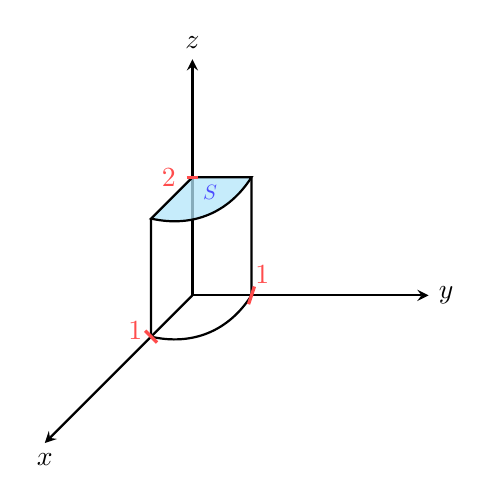
\begin{tikzpicture}[scale=1.5]
                \draw[thick,-stealth] (0,0) -- (-1.25,-1.25) node[anchor=north] {$x$};
                \draw[thick,-stealth] (0,0) -- (2,0) node[anchor=west] {$y$};
                \draw[thick,-stealth] (0,0) -- (0,2) node[anchor=south] {$z$};
                \draw[thick] (0.5,1) -- (0.5,0) to[bend left=35] (-0.35,-0.35) -- (-0.35,0.65);
                \draw[thick, fill=cyan!30,fill opacity=0.75] (0,1) -- (0.5,1) node[midway,below,xshift=-0.15cm,opacity=1,scale=0.75,blue!70] {$S$}to[bend left=35] (-0.35,0.65) -- cycle;
                \draw[very thick, red!70] (0.525,0.075) node[anchor=south west,xshift=-0.125cm,yshift=-0.1cm] {$1$} -- (0.475,-0.075);
                \draw[very thick, red!70] (-0.4,-0.3) node[anchor=east,xshift=0.1cm] {$1$} -- (-0.3,-0.4);
                \draw[very thick, red!70] (-0.05,1) node[anchor=east] {$2$} -- (0.05,1);
            \end{tikzpicture}
        \end{center}
        \begin{solution}
            The divergence theorem says:
            \[ \iint_S \mathbf V \cdot \hat n \ dA = \iiint_E \div \mathbf V d\mathcal V\]
            For the right hand side, we can compute the volume integral:
            \begin{align*}
                \iiint_E (\div \mathbf V) d\mathcal V &= \int_0^1 \int_0^{\pi/2} \int_0^2 \left(2\cos^2 \phi + \cos(2\phi) + 7\right)\cdot s dz d\phi ds\\
                &= \int_0^1 \int_0^{\pi/2} s(4\cos^2 \phi + 2\cos(2\phi) + 7) d\phi ds\\
                &=  \int_0^1 s(4\frac{\pi}{4} + 2(0) + 7\pi) ds\\
                &= \frac{8\pi}{2} = 4\pi
            \end{align*}
            To compute the surface integral, we have to break it up into 5 segments: the two caps, the curved surface, and the two surfaces along the axes. First, we calculate the two caps. 

            Notice that for the caps, $\hat n = (0, 0, 1)$, so we only take the $\hat z$ comopnent of $\mathbf V$. Our bounds of integration are from $\phi \in [0, \pi/2]$ and $s \in [0, 1]$. First, we calculate the bottom cap:
            \[ s_1 = \int_0^1 \int_0^{\pi/2} 3sz \ d\phi ds\]
            But $z = 0$, so we get $s_1 = 0$.

            For the top cap, we have $z = 2$, so therefore
            \[ s_2 = \int_0^1 \int_0^{\pi/2} 6s \ d\phi ds = \int_0^1 3\pi s \ ds = \frac{3\pi}{2}\]

            Now we compute the curved surface $s_3$. Here, we have $\phi \in [0, \pi/2]$ and $z \in [0, 2]$, $s = 1$ and $\hat n = (1, 0, 0)$ is $(1, 0, 0)$, so we only take the $\hat s$ component of $\mathbf V$. Therefore:
            \[ s_3 = \int_0^2 \int_0^{\pi/2}(2 + \cos^2 \phi)s \ d\phi dz = \int_0^2 2 \cdot \frac{\pi}{2} + \frac{\pi}{4} = \frac{5\pi}{2}\]
            Now we take a look at the two sides on the axes. For the plane on the $xz$-plane, we have $s \in [0, 1]$, $z \in [0, 2]$, $\hat n = (0, -1, 0)$ and $\phi = 0$. Therefore:
            \[ s_4 = -\int_0^1 \int_0^2 s^2 \sin \phi \cos \phi \ dz ds\]
            But notice that since $\phi = 0$, then $\sin \phi = 0$ and so therefore $s_4 = 0$. 

            A similar story exists with the other side: the integration bounds are the same and $\hat n = (0, 1, 0)$, $\phi = \pi/2$. Therefore: 
            \[ s_5 = \int_0^1 \int_0^2 s^2 \sin \phi \cos \phi \ dz ds\] 
            But since $\phi = \pi/2$, then $\cos \phi = 0$, and so therefore $s_5 = 0$ as well. Now we can finally take the sum of all of them:
            \[ \iint_S \mathbf V \cdot n dA = s_1 + s_2 + s_3 + s_4 + s_5 = \frac{3\pi}{2} + \frac{5\pi}{2} = 4\pi\] 
            which equals what we calculated on the right hand side, as desired.
        \end{solution}
        \item Verify that Stoke's theorem holds true using the surface $S$ shown in the figure below.
        
        \begin{solution}
            Stokes' theorem says 
            \[ \oint_S \mathbf V \cdot dl = \iint_S (\curl \mathbf V)\  dA\]
            Computing the right hand side of this integral, the region is defined by $s \in [0, 1], \phi \in [0, \pi/2]$ and $z = 2$, with $\hat n = (0, 0, 1)$, so therefore: 

            \[ \iint_S \curl \mathbf V \ dA = \int_0^1 \int_0^{\pi/2} 2\sin(2\phi)s \ d\phi ds = 2\int_0^1 s ds = 1\]
            
            To compute the left hand side, we split up the integral into three different parts. We split this into three segments, revolving counterclockwise around the surface. 

            The first segment has $r \in [0, 1]$ with $\phi = 0$ and $z = 2$, so this gives:
            \[ s_1 = \int_0^1 s(2 + \cos^2 \phi) ds = \int_0^1 3s \ ds = \frac 32\]
            The second segment has $r = 1, \phi \in [0, \pi/2], z = 2$, so 
            \[ s_2 = \int_0^{\pi/2} \sin \phi \cos \phi \cdot s \ d\phi = \frac 12\]
            The final segment has $r \in [0, 1]$, $\phi = \pi/2$ and $z = 2$, but we have to take the integral from $r = 1 \to r = 0$ because we need to preserve direction:
            \[ s_3 = \int_1^0 s(2 + \cos^2 \phi) \ ds = \int_1^0 2s \ ds = -1\]
            And so the total is:
            \[ S = \frac 32 + \frac 12 - 1 = 1\] 
            which is what we obtained on the right hand side, so we're done.
        \end{solution}
    \end{enumerate}

    \pagebreak

    \section*{Problem 2}
    The vector field 

    \[ \mathbf E = \frac{p}{4\pi \epsilon_0 r^3}\left( 2 \cos \theta \hat r + \sin \theta \hat \theta\right) - \frac{\mathbf p}{3\epsilon_0} \delta^3(r)\] 
    where $p$ is a constant in the $z$-direction, can be written as a gradient of some scalar function $V(r)$. Find the scalar functi $V(r)$ for $r \neq 0$. 
    \textit{Note:} The second term including the delta function is added for completeness, but you do not need to worry aboutit here. I do NOT recommend you using the Helmholtz theorem where 
    \[ V(r) = \frac{1}{4\pi} \int_{\mathbb R^3} \frac{\div \mathbf E}{\rcurs} d\tau'\]
    because the divergence at the origin is very tricky to deal with as it's not mathematically well-defined. Instead, thikn of this problme as solving the differential equation $\mathbf E = -\nabla V$ for $r \neq 0$

    \begin{solution}
        Again, we know that the gradient of a scalar function $T$ is written as 
        \[ \nabla T = \pdv{T}{r} \hat r + \frac 1r \pdv{T}{\theta}\hat \theta + \frac{1}{r\sin \theta} \pdv{T}{\phi} \hat \phi\]
        We don't have a $\phi$ component in this case, so we instead just solve: 
        \[ -\pdv{V}{r} \hat r = \frac{2p \cos \theta}{4\pi \epsilon_0 r^3} \hat r = \frac{p \cos \theta}{2\pi \epsilon_0 r^3}\]
        Integrating this with respect to $r$, we get:
        \[ V = \frac 12 \frac{p \cos \theta}{2\pi \epsilon_0 r^2}\hat r + g(\theta)\] 
        We have to insert $g(\theta)$ here for compleness, since its partial derivative with respect to $r$ is 0. Now taking the derivative with respect to $\theta$: 
        \[ -\frac 1r \pdv{V}{\theta} = \frac{p}{4\pi \epsilon_0 r^3} \cdot (-\sin \theta) + g'(\theta) \implies g'(\theta) = 0\]
        And so therefore:
        \[ V(r, \theta) = \frac{p \cos \theta}{4\pi \epsilon_0 r^2}\]
        For the $\hat z$ direction, we have:
        \[ -\pdv{V}{z} = -\frac{\mathbf p}{3\epsilon} \delta^3(r)\]
        so integrating we get:
        \[ V_z = \frac{\mathbf p z}{3\epsilon_0} \delta^3(r)\]
        So finally we have
        \[ V = \frac{p \cos \theta}{4\pi \epsilon_0 r} + \frac{\mathbf p z}{3\epsilon_0}\delta^3(r)\]
    \end{solution}

    \pagebreak

    \section*{Problem 3}
    Show the following integral theorems: 
    \begin{enumerate}[label=(\alph*)]
        \item $\displaystyle \int_{\mathcal V} (\nabla T) d\tau =\displaystyle \oint_S T d \mathbf a$
        \item $\displaystyle \int_{\mathcal V} (\curl \mathbf V) d\tau = -\displaystyle \oint_{\mathcal S} \mathbf V \times d\mathbf a$
        \item $\displaystyle \int_{\mathcal V} (T \nabla^2 U - U \nabla^2 T) d\tau = \displaystyle \oint_S (T \nabla U - U \nabla T) \cdot d\mathbf a$
    \end{enumerate}
    Here $\mathcal V$ is a three-dimensional region in 3D flat space and $\mathcal S$ is its boundary. $T, U$ are scalar fields, while $\mathbf V$ is a vector field. For (a), you can use the divergence theorem but with the vector field to be $\mathbf cT$ where $\mathbf c$ is a constant vector field. For (b), you can again consider divergence theorem but with the vector field to be $\mathbf {V \times c}$ where again $\mathbf c$ is a constant vector field.

    \begin{solution}
        \begin{enumerate}[label=(\alph*)]
            \item From the divergence theorem, we know that 
            \[ \int_{\mathcal V} \div T = \int_{\partial \mathcal V} T dS\]
            Now, take the vector field to be $\mathbf cT$ where $\mathbf c$ is a constant vector field. Therefore: 
            \begin{align*}
                \mathbf c \cdot \int_{\mathcal V} (\nabla T) d\tau &= \int_{\mathcal V} \mathbf c \nabla T \ d\tau\\
                &= \int_{\mathcal V} \nabla (\mathbf cT) - \int_{\mathcal V} T(\div \mathbf c) d \tau\\
                &=\int_{\partial \mathcal V} T \mathbf c \cdot d\mathbf a\\
                &= \mathbf c \cdot \int_{\partial \mathcal V} T \ d \mathbf a = \mathbf c \cdot \oint_S T d\mathbf a
            \end{align*}
            here $\mathbf c$ is on both sides of the equation, so we can safely say that 
            \[ \int_{\mathcal V} (\nabla T) \cdot T = \oint_{\mathcal S} T \cdot d\mathbf a\]
            as desired. 
            \item Using the hint again, we let $T = \mathbf V \times \mathbf c$ where $\mathbf c$ is a constant vector field:
            \begin{align*}
                \int_{\mathcal V}(\div (\mathbf {V \times c})) \ d\tau &= \oint_{\mathcal S} (\mathbf{V \times c}) d \mathbf a \\
                &= \int_{\mathcal V} (\curl \mathbf V) \cdot \mathbf c - \mathbf V \cdot \underbrace{(\curl \mathbf c)}_{= 0} \ d\tau\\
                &= \int_{\mathcal V} (\curl \mathbf  V) \cdot \mathbf c \ d\tau\\
                &= \oint_{\mathcal S} (\mathbf {V \times c}) \cdot d\mathbf a\\
                &= \oint_{\mathcal S} \mathbf c \cdot (d\mathbf{a \times V}) \\
                &= \mathbf c \cdot \left(-\oint_{\mathcal S} \mathbf V \times d\mathbf a\right)
            \end{align*}
            And so now we've derived the relation:
            \[ \mathbf c \cdot \int_{\mathcal V} (\curl \mathbf V)\ d\tau = \mathbf c \cdot (-\oint_S \mathbf V \cdot d\mathbf a)\] 
            and since $\mathbf c$ exists on both sides, thne we can say:
            \[ \int_{\mathcal{V}}(\curl\mathbf{V})d\tau = -\oint_{\mathcal{S}}\mathbf{V}\times d\mathbf{a}\] 
            As desired.

            \item From the first part, we know that 
            \[ \int_{\mathcal V} \nabla F \ d\tau = \oint_{\mathcal S} F \ d\mathbf a\]
            So in this problem, we will let $F = T \nabla U - U \nabla T$ so we can use this theorem and obtian the left hand side. Computing the gradient: 
            \[ \nabla F = T \nabla^2 U - \nabla T \nabla U - \nabla U \nabla T - U \nabla^2 T\] 
            and since gradients commute, then 
            \[ \nabla F = T \nabla^2 U - U\nabla^2 T\] 
            So therefore:
            \[ \int_{\mathcal V} (T \nabla^2 U - U \nabla^2 T) \ d\tau = \oint_{\mathcal S}(T \nabla U - U\nabla T) \cdot d\mathbf a\]
            as desired.
        \end{enumerate}
    \end{solution}
\end{document}